\documentclass[12pt,a4paper,twoside]{memoir}
\usepackage[utf8]{inputenc}
\usepackage{graphicx}
\author{Robert James}
\title{Interfaces in the 2D Potts model}

\begin{document}

\maketitle

% begin abstract
\begin{abstract}

\end{abstract}
% end abstract

\tableofcontents

% begin Introduction
\chapter{Introduction}
%Give basic idea of the project and its content. Describe (and give references to) other relevant work in the literature.
In the field of Computational Physics, there is a large interest in lattice simulation.
One of the most simple models that still exhibits non trivial behaviour is the q-state Potts Model.
By Restricting the Potts model to 2 dimensions and the number of independent states,$q = 2$ you can determine the behaviour at high,low and critical temperatures analytically \cite{Montroll1963}this is known as the Ising Model.

% end Introduction

% begin Theory
\chapter{Theory}
%Necessary theoretical background

\section{Thermodynamic Limit}
In the thermodynamic limit,
\begin{equation}
	N\rightarrow\infty, V\rightarrow\infty, \frac{N}{V} = const.
\end{equation}

As stated earlier in computer simulations the concept of $\infty$ is completely redundant.
Computers retain a restricted amount of memory available to perform calculations.
To this end, simulations in general study the behaviour of smaller systems.
Depending on the complexity of the problems invovled and how co-related each site is, you often find a large range in sizes from $8x8$ up to several thousand.
Assuming momentarilly you could perform computer simulations for an inifinite lattice, you would find results that after reasonable thermalisation and statistical analysis that are identical to a theoretical prediction.
As stated earlier, the number of lattice sites you can reasonablly use for simulation purposes is restricted.
This introduces boundary effects and noise that are not present on an inifite grid.
To reduce this problem you turn to your lattice construction.

\section{Lattice}
As stated earlier, it is impossible to perform computer simulations for inifite lattice sizes.
By shrinking the lattices down to useable sizes you typically introduce boundary effects that can add a layer of noise to the data.
To reduce the effects of boundary noise, you can enforce periodic boundary conditions on your lattice such that
\begin{equation}
	\begin{split}
		s_{i=L,j=0} = s_{i=0,j=0}  \\
		s_{i=0,j=L} = s_{i=0,j=0}
	\end{split}
\end{equation}
In a physical sense taking a 2 dimensional lattice and enforcing such boundary conditions upon it leads to a torus as shown below.
\begin{figure}[h!]
	\centering
	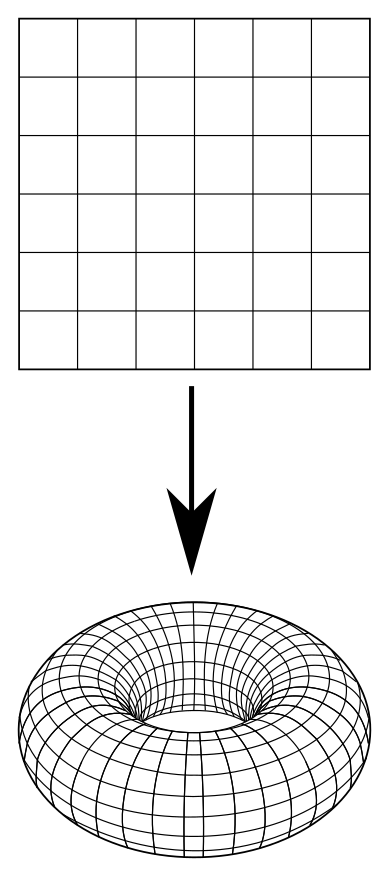
\includegraphics[width=0.25\textwidth]{2-Theory/latticetotorus.png}
	\caption{2 dimensional lattice transforming to torus under periodic boundary conditions}
\end{figure}

\section{Interfaces}

\section{Observables}
	\subsection{Magnetisation}
	Materials are often classified by their responses to externally applied fields.
	The types of response to the applied fields are diamagnetic, paramagnetic or ferromagnetic.
	Diamagnetism is the weakest response and opposes the applied magnetic field.
	Paramagnetism is stronger than diamagnetism and is proportional to the field strength and aligned to the direction.
	Ferromagnetism, is the type of magnetism studied in this project, the effects of this type of response can occasionally be orders of magntitude larger than of the other types.
	In this project, we have no externally applied field.
	Diamagnetism and Paramagnetism in this case do not apply because they are in response to an externally applied field.
	\begin{equation}
		M=\sum_{i}^{V}\sigma_{i}
	\end{equation}

	\subsection{Energy}
	\begin{equation}
		H=E=-\sum_{i,j}\delta (\sigma_i,\sigma_j)
	\end{equation}

	\subsection{Specific Heat}
	\begin{equation}
		C=\beta^2[<E^2>-<E>^2]
	\end{equation}

	\subsection{Magnetic Susceptibility}
	\begin{equation}
		\chi=\beta[<M^2>-<M>^2]
	\end{equation}

\section{Partition Function}

	\subsection{Calculating the DoS}

\section{Fixing the Partition Functions}

\section{Free Energy}

% end Theory

% begin Code
\chapter{Code}
% end Code

% begin Results
\chapter{Results}
% end Results

% begin DiscussionofResults
\chapter{Discussion of Results}
% end DiscussionofResults

% begin Conclusions
\chapter{Conclusion and Reflection}
Wibble Wobble
% end Conclusions

% begin Appendices
\chapter{Appendices}
\section{Program Source Code}
\subsection{main.cpp}
\lstinputlisting[language=C++,breaklines=true]{7-Appendices/main.cpp}

\subsection{utilityfunctions.cpp}
\lstinputlisting[language=C++,breaklines=true]{7-Appendices/utilityfunctions.cpp}

\subsection{potts.cpp}
\lstinputlisting[language=C++,breaklines=true]{7-Appendices/potts.cpp}

\subsection{metropolis.cpp}
\lstinputlisting[language=C++,breaklines=true]{7-Appendices/metropolis.cpp}

\subsection{wanglandau.cpp}
\lstinputlisting[language=C++,breaklines=true]{7-Appendices/wanglandau.cpp}


\section{Metropolis}
\subsection{Q10EnergyBeta16x16RangeofBeta.dat}
\begin{lstlisting}
0 -0.200109 0.00025786
0.05 -0.209624 0.00027772
0.1 -0.21899 0.000264747
0.15 -0.22827 0.000328895
0.2 -0.239697 0.00034315
0.25 -0.249341 0.000322799
0.3 -0.260898 0.000375688
0.35 -0.272723 0.000393963
0.4 -0.284388 0.000390524
0.45 -0.297082 0.000406967
0.5 -0.311139 0.000454669
0.55 -0.324349 0.000481373
0.6 -0.339617 0.000556149
0.65 -0.355262 0.000571083
0.7 -0.370582 0.000588718
0.75 -0.388206 0.000693746
0.8 -0.404432 0.000805053
0.85 -0.423668 0.000777047
0.9 -0.44452 0.000851305
0.95 -0.465189 0.000954719
1 -0.49025 0.00117225
1.05 -0.516876 0.00126606
1.1 -0.546703 0.00145358
1.15 -0.57747 0.0017864
1.2 -0.611437 0.00197478
1.25 -0.650466 0.00275758
1.3 -0.696883 0.00279037
1.35 -0.772292 0.00896837
1.4 -0.948917 0.0261211
1.45 -1.77709 0.00725456
1.5 -1.83122 0.00498143
1.55 -1.87696 0.00297309
1.6 -1.91116 0.00235711
1.65 -1.93321 0.00199471
1.7 -1.94931 0.00146225
1.75 -1.95923 0.00132297
1.8 -1.96639 0.00101562
1.85 -1.97237 0.001026
1.9 -1.97907 0.000982634
1.95 -1.98302 0.000793976
2 -1.98726 0.000609572
2.05 -1.98861 0.000599667
2.1 -1.99062 0.000576544
2.15 -1.99192 0.000539044
2.2 -1.99415 0.000428889
2.25 -1.9955 0.00038934
2.3 -1.99605 0.000289569
2.35 -1.99703 0.000253472
2.4 -1.99816 0.000224678
2.5 -1.99819 0.000216858
2.55 -1.99873 0.000179629
2.6 -1.99891 0.000202063
2.65 -1.99915 0.000155375
2.7 -1.99914 0.000163213
2.75 -1.99921 0.000150579
2.8 -1.99939 0.000147808
\end{lstlisting}

\subsection{Q10MagnetisationBeta16x16RangeofBeta.dat}
\begin{lstlisting}
0 0.0536258 0.000282599
0.05 0.0540781 0.000279901
0.1 0.0542501 0.000287509
0.15 0.0554078 0.000295225
0.2 0.0564436 0.000321571
0.25 0.0566199 0.000357871
0.3 0.0576936 0.000371024
0.35 0.0579753 0.000341963
0.4 0.0585935 0.000385968
0.45 0.0603006 0.000411977
0.5 0.0615635 0.000414219
0.55 0.0630296 0.000409879
0.6 0.0633744 0.000417007
0.65 0.0654273 0.000408695
0.7 0.0667299 0.000475517
0.75 0.06832 0.000532082
0.8 0.0693393 0.000636549
0.85 0.0719688 0.00063416
0.9 0.0744893 0.000661863
0.95 0.0769229 0.000845882
1 0.0786101 0.000861817
1.05 0.083604 0.000845359
1.1 0.0866739 0.00114479
1.15 0.0903927 0.00144828
1.2 0.0996223 0.00169752
1.25 0.105431 0.00180421
1.3 0.114108 0.00265604
1.35 0.14669 0.00880269
1.4 0.260539 0.0227491
1.45 0.916998 0.00384802
1.5 0.940809 0.00234376
1.55 0.958311 0.00120807
1.6 0.970224 0.000934043
1.65 0.977959 0.000659634
1.7 0.983036 0.000501082
1.75 0.986376 0.000447583
1.8 0.988708 0.000321665
1.85 0.990527 0.000337317
1.9 0.992693 0.00032042
1.95 0.993967 0.000271542
2 0.995432 0.000211862
2.05 0.99583 0.000202744
2.1 0.996618 0.000202872
2.15 0.997036 0.000191388
2.2 0.997793 0.000166809
2.25 0.995348 7.58233e-05
2.3 0.998512 0.000107969
2.35 0.995623 4.63501e-05pn
2.4 0.9993 8.78052e-05
2.5 0.999318 7.76653e-05
2.55 0.999527 6.85556e-05
2.6 0.999585 7.80653e-05
2.65 0.999671 6.15873e-05
2.7 0.999652 6.92973e-05
2.75 0.995975 2.34157e-05
2.8 0.999773 5.52442e-05
\end{lstlisting}

\subsection{Q10SpecificHeatBeta16x16RangeofBeta.dat}
\begin{lstlisting}
0 0 0.000277831
0.05 1.83835e-06 0.000301732
0.1 7.59666e-06 0.000289046
0.15 1.8079e-05 0.000362044
0.2 3.32178e-05 0.000381555
0.25 5.3092e-05 0.000361097
0.3 8.05329e-05 0.000424603
0.35 0.000116444 0.00045009
0.4 0.000153867 0.000448959
0.45 0.000200627 0.000474747
0.5 0.000266681 0.000538302
0.55 0.00033652 0.000575057
0.6 0.000424915 0.000675175
0.65 0.000509799 0.000702659
0.7 0.000625063 0.000735869
0.75 0.000778356 0.000885296
0.8 0.000890101 0.00104076
0.85 0.00114436 0.00102571
0.9 0.00135769 0.00114159
0.95 0.00157159 0.00131239
1 0.00188835 0.00166014
1.05 0.0023751 0.00183388
1.1 0.00278538 0.00217225
1.15 0.00348612 0.00274892
1.2 0.00416383 0.00314387
1.25 0.00556986 0.0046199
1.3 0.00643498 0.00486409
1.35 0.0214081 0.0186271
1.4 0.140861 0.0700809
1.45 0.0178388 0.0262297
1.5 0.010962 0.0184243
1.55 0.00702258 0.0114387
1.6 0.00515308 0.00921808
1.65 0.00358491 0.00791604
1.7 0.00256486 0.00585533
1.75 0.00220429 0.00532126
1.8 0.00170033 0.00410681
1.85 0.00164258 0.00415803
1.9 0.0013511 0.00399262
1.95 0.00107063 0.00323329
2 0.000802398 0.00249073
2.05 0.000762133 0.00244968
2.1 0.000673591 0.00235798
2.15 0.000638553 0.00220467
2.2 0.000472682 0.00175664
2.25 0.000351523 0.00159687
2.3 0.000319642 0.00118773
2.35 0.00025569 0.00103987
2.4 0.000164989 0.000922352
2.5 0.000177274 0.000889706
2.55 0.000121696 0.000737807
2.6 0.000113462 0.000829744
2.65 0.000100027 0.000637751
2.7 9.9788e-05 0.000670199
2.75 9.32963e-05 0.000618449
2.8 7.96827e-05 0.000606782
\end{lstlisting}
\subsection{Q10SusceptibilityBeta16x16RangeofBeta.dat}
\begin{lstlisting}
0 0 0.00028509
0.05 4.29466e-05 0.000282763
0.1 8.58881e-05 0.000290136
0.15 0.000135661 0.000298115
0.2 0.000184004 0.000325097
0.25 0.000230868 0.00036167
0.3 0.000297625 0.00037515
0.35 0.000341974 0.000345617
0.4 0.000402675 0.000390005
0.45 0.000479985 0.000416988
0.5 0.000555462 0.000419142
0.55 0.000639779 0.000415187
0.6 0.000702171 0.000422092
0.65 0.000797168 0.000414669
0.7 0.000880077 0.000481797
0.75 0.000993099 0.000539691
0.8 0.00109877 0.000646136
0.85 0.00125121 0.000643803
0.9 0.00138957 0.000673981
0.95 0.00166783 0.000861908
1 0.00178388 0.000879005
1.05 0.00208251 0.000864356
1.1 0.0023205 0.00116932
1.15 0.00272497 0.00148544
1.2 0.00330586 0.00174601
1.25 0.00370356 0.00185931
1.3 0.00485822 0.0027615
1.35 0.0158726 0.010339
1.4 0.0781662 0.0319328
1.45 0.00324901 0.00774562
1.5 0.00153613 0.00483858
1.55 0.000770371 0.00257786
1.6 0.000535052 0.00201244
1.65 0.000292019 0.00144091
1.7 0.000207642 0.00110016
1.75 0.000169414 0.000984836
1.8 0.00012585 0.000710757
1.85 0.000119812 0.000746123
1.9 9.35882e-05 0.000710222
1.95 7.74758e-05 0.000602487
2 5.65397e-05 0.000471058
2.05 5.37267e-05 0.000450788
2.1 4.51293e-05 0.000451287
2.15 4.36806e-05 0.00042575
2.2 3.4398e-05 0.000371114
2.25 9.52731e-06 0.000168444
2.3 2.20644e-05 0.000240564
2.35 5.39795e-06 0.000103016
2.4 1.10412e-05 0.000195722
2.5 1.11168e-05 0.00017311
2.55 7.38777e-06 0.000152878
2.6 7.03322e-06 0.000174046
2.65 6.69305e-06 0.000137209
2.7 6.75523e-06 0.000154427
2.75 1.38085e-06 5.20999e-05
2.8 4.30191e-06 0.000123173
\end{lstlisting}

\section{Wang Landau}
\subsection{An16x16Convergence.dat}
\begin{lstlisting}
2
1.83742
1.67596
1.51659
1.36017
1.21047
1.07115
0.958293
0.898123
0.886636
0.894645
0.890632
0.876113
0.886485
0.882993
0.893742
0.900179
0.882147
0.896148
0.885572
0.890101
0.889612
0.930086
0.897667
0.886961
0.885495
0.895436
0.889006
0.904736
0.884794
0.88835
0.894414
0.906143
0.885411
0.893166
0.895981
0.892837
0.896723
0.888887
0.888455
0.889703
0.896108
0.891426
0.891259
0.884917
0.882937
0.888925
0.889294
0.879971
0.887493
0.885633
0.881775
0.912052
0.894377
0.885789
0.886023
0.890293
0.887923
0.886067
0.881623
0.883337
0.879752
0.888423
0.885911
0.8877
0.881466
0.908074
0.889962
0.88437
0.890146
0.890344
0.881311
0.923801
0.895426
0.887581
0.883116
0.887668
0.883806
0.893626
0.890971
0.886484
0.885689
0.888526
0.885702
0.888504
0.895164
0.892044
0.879771
0.892959
0.900478
0.888948
0.887261
0.888088
0.894206
0.901281
0.885127
0.896582
0.896501
0.90774
0.880374
\end{lstlisting}

\subsection{Continuity Constants}
\label{subsec:ContinuityConstants}

\left(
\begin{array}{ccccc}
\centering
 Q2 & Q3 & Q4 & Q8 & Q10 \\
 \hline
 0.0783575 & 0.0887444 & 0.0948331 & 0.107823 & 0.112169 \\
 0.149986 & 0.170668 & 0.182925 & 0.209201 & 0.217729 \\
 0.212082 & 0.242924 & 0.261318 & 0.301153 & 0.313728 \\
 0.269831 & 0.310671 & 0.335173 & 0.38864 & 0.405326 \\
 0.325173 & 0.375721 & 0.40646 & 0.473809 & 0.494806 \\
 0.378996 & 0.439152 & 0.47602 & 0.557657 & 0.583087 \\
 0.431435 & 0.501496 & 0.544567 & 0.640646 & 0.670586 \\
 0.481899 & 0.562968 & 0.61251 & 0.723112 & 0.75776 \\
 0.529428 & 0.623959 & 0.679999 & 0.805459 & 0.844962 \\
 0.573241 & 0.684446 & 0.74747 & 0.887795 & 0.932316 \\
 0.612643 & 0.743848 & 0.814892 & 0.970099 & 1.01998 \\
 0.647018 & 0.801437 & 0.881851 & 1.05277 & 1.10781 \\
 0.675715 & 0.856414 & 0.947792 & 1.1361 & 1.19608 \\
 0.69803 & 0.908095 & 1.0121 & 1.21999 & 1.28512 \\
 0.713377 & 0.955984 & 1.0742 & 1.30418 & 1.37436 \\
 0.721189 & 0.999568 & 1.13333 & 1.3882 & 1.46418 \\
 \text{Null} & 1.03814 & 1.189 & 1.4716 & 1.55451 \\
 \text{Null} & 1.07098 & 1.24065 & 1.55375 & 1.64428 \\
 \text{Null} & 1.09738 & 1.28747 & 1.63399 & 1.73275 \\
 \text{Null} & 1.11655 & 1.32871 & 1.71175 & 1.81937 \\
 \text{Null} & 1.12791 & 1.36349 & 1.78614 & 1.9035 \\
 \text{Null} & \text{Null} & 1.39094 & 1.85622 & 1.98427 \\
 \text{Null} & \text{Null} & 1.41012 & 1.92089 & 2.06066 \\
 \text{Null} & \text{Null} & 1.42016 & 1.97909 & 2.13154 \\
 \text{Null} & \text{Null} & \text{Null} & 2.02948 & 2.19551 \\
 \text{Null} & \text{Null} & \text{Null} & 2.0704 & 2.25085 \\
 \text{Null} & \text{Null} & \text{Null} & 2.10006 & 2.29553 \\
 \text{Null} & \text{Null} & \text{Null} & 2.11625 & 2.32719 \\
 \text{Null} & \text{Null} & \text{Null} & \text{Null} & 2.34277 \\
 \text{Null} & \text{Null} & \text{Null} & \text{Null} & \text{Null} \\
 \text{Null} & \text{Null} & \text{Null} & \text{Null} & \text{Null} \\
 \text{Null} & \text{Null} & \text{Null} & \text{Null} & \text{Null} \\
\end{array}
\right)

\subsection{Q2 Piecewise Function}
\label{subsec:Q2Piecewise}
\begin{array}{cc}
\centering
 1.25372 (x+1.96875)+0.0783575 & -2\leq x\leq -1.9375 \\
 1.03838 (x+1.90625)+0.149986 & -1.9375\leq x\leq -1.875 \\
 0.948715 (x+1.84375)+0.212082 & -1.875\leq x\leq -1.8125 \\
 0.899257 (x+1.78125)+0.269831 & -1.8125\leq x\leq -1.75 \\
 0.87168 (x+1.71875)+0.325173 & -1.75\leq x\leq -1.6875 \\
 0.85064 (x+1.65625)+0.378996 & -1.6875\leq x\leq -1.625 \\
 0.827427 (x+1.59375)+0.431435 & -1.625\leq x\leq -1.5625 \\
 0.787394 (x+1.53125)+0.481899 & -1.5625\leq x\leq -1.5 \\
 0.733548 (x+1.46875)+0.529428 & -1.5\leq x\leq -1.4375 \\
 0.668473 (x+1.40625)+0.573241 & -1.4375\leq x\leq -1.375 \\
 0.592389 (x+1.34375)+0.612643 & -1.375\leq x\leq -1.3125 \\
 0.507607 (x+1.28125)+0.647018 & -1.3125\leq x\leq -1.25 \\
 0.410693 (x+1.21875)+0.675715 & -1.25\leq x\leq -1.1875 \\
 0.303397 (x+1.15625)+0.69803 & -1.1875\leq x\leq -1.125 \\
 0.187714 (x+1.09375)+0.713377 & -1.125\leq x\leq -1.0625 \\
 0.0622752 (x+1.03125)+0.721189 & -1.0625\leq x\leq -1 \\
\end{array}

\subsection{Q3 Q4 Q8 Q10 $Log(g(E))$}
\label{subsec:QLogg}
\begin{figure}[H]
\centering
\begin{subfigure}[b]{0.45\textwidth}
    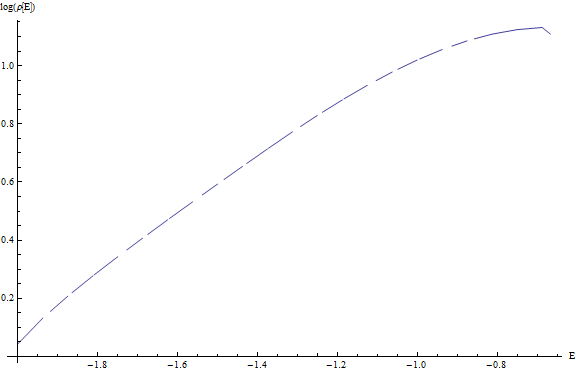
\includegraphics[width=\textwidth]{7-Appendices/Q3Log(rho(E)).png}
    \caption{Graph showing the $\log{g\left(E\right)}$ vs E for Q3}
\end{subfigure}
\begin{subfigure}[b]{0.45\textwidth}
    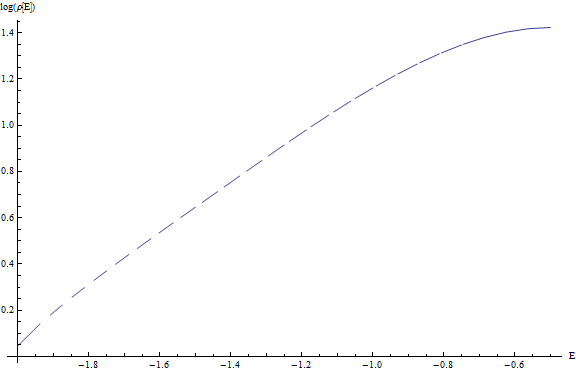
\includegraphics[width=\textwidth]{7-Appendices/Q4Log(rho(E)).png}
    \caption{Graph showing the $\log{g\left(E\right)}$ vs E for Q4}
\end{subfigure}

\begin{subfigure}[b]{0.45\textwidth}
    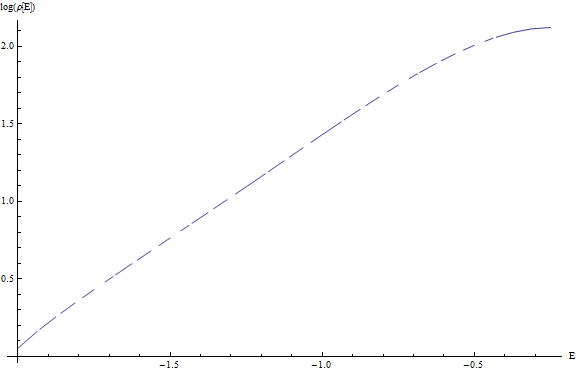
\includegraphics[width=\textwidth]{7-Appendices/Q8Log(rho(E)).png}
    \caption{Graph showing the $\log{g\left(E\right)}$ vs E for Q8}
\end{subfigure}
\begin{subfigure}[b]{0.45\textwidth}
    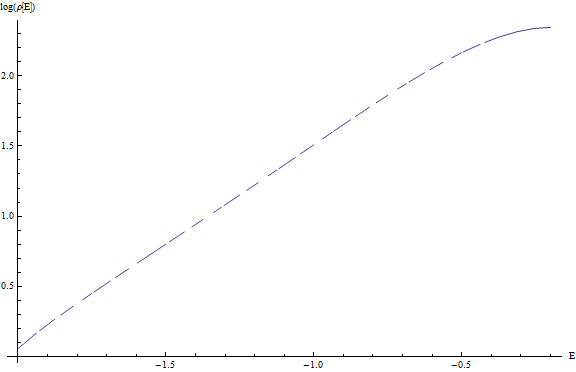
\includegraphics[width=\textwidth]{7-Appendices/Q10Log(rho(E)).png}
    \caption{Graph showing the $\log{g\left(E\right)}$ vs E for Q10}
\end{subfigure}
\end{figure}

\subsection{Q3 Q4 Q8 Q10 $Log(g(E))$ Twisted}
\label{subsec:QLoggInt}
\begin{figure}[H]
\centering
\begin{subfigure}[b]{0.45\textwidth}
    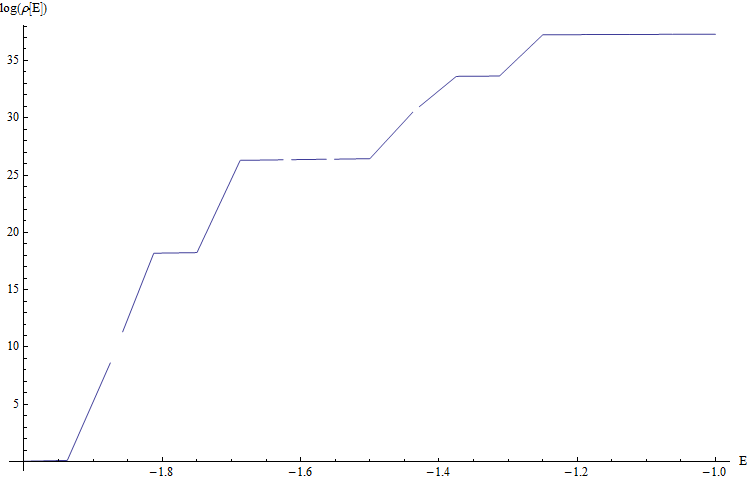
\includegraphics[width=\textwidth]{7-Appendices/intQ2Log(rho(E)).png}
    \caption{Graph showing the $\log{g\left(E\right)}$ vs E for Q2}
\end{subfigure}
\begin{subfigure}[b]{0.45\textwidth}
    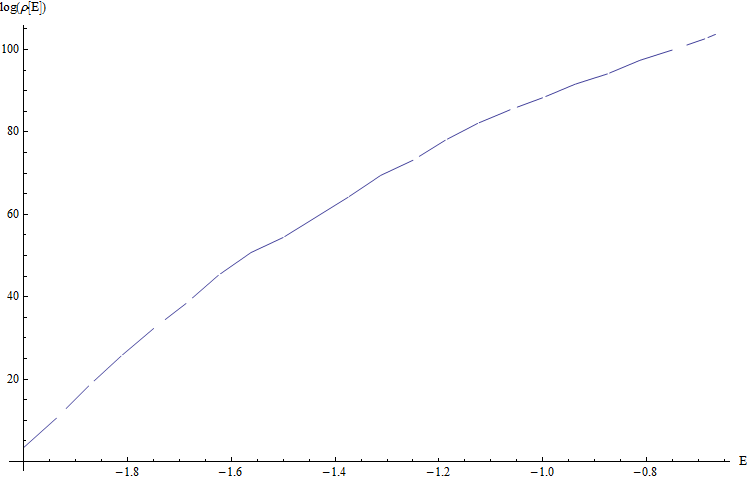
\includegraphics[width=\textwidth]{7-Appendices/intQ3Log(rho(E)).png}
    \caption{Graph showing the $\log{g\left(E\right)}$ vs E for Q3}
\end{subfigure}

\begin{subfigure}[b]{0.45\textwidth}
    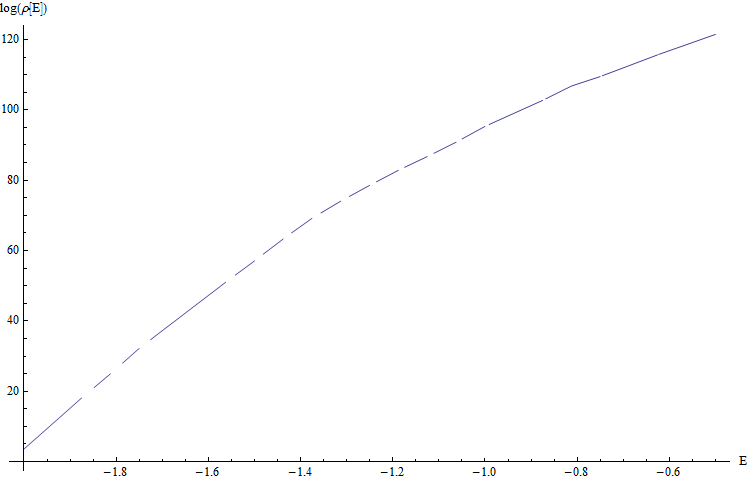
\includegraphics[width=\textwidth]{7-Appendices/intQ4Log(rho(E)).png}
    \caption{Graph showing the $\log{g\left(E\right)}$ vs E for Q4}
\end{subfigure}

\begin{subfigure}[b]{0.45\textwidth}
    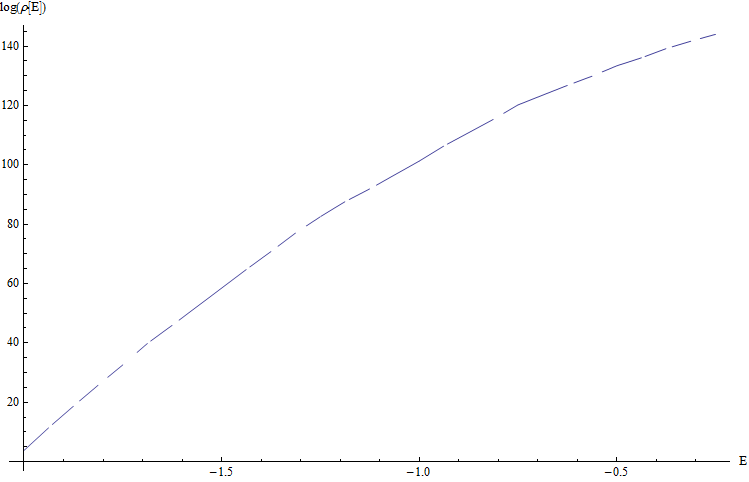
\includegraphics[width=\textwidth]{7-Appendices/intQ8Log(rho(E)).png}
    \caption{Graph showing the $\log{g\left(E\right)}$ vs E for Q8}
\end{subfigure}
\begin{subfigure}[b]{0.45\textwidth}
    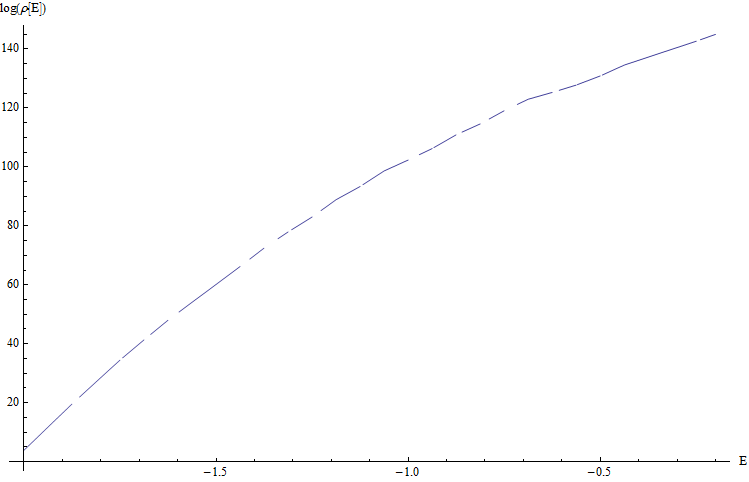
\includegraphics[width=\textwidth]{7-Appendices/intQ10Log(rho(E)).png}
    \caption{Graph showing the $\log{g\left(E\right)}$ vs E for Q10}
\end{subfigure}
\end{figure}

\subsection{Mathematica Data Processing Notebook}
\label{subsec:MathematicaNotebook}
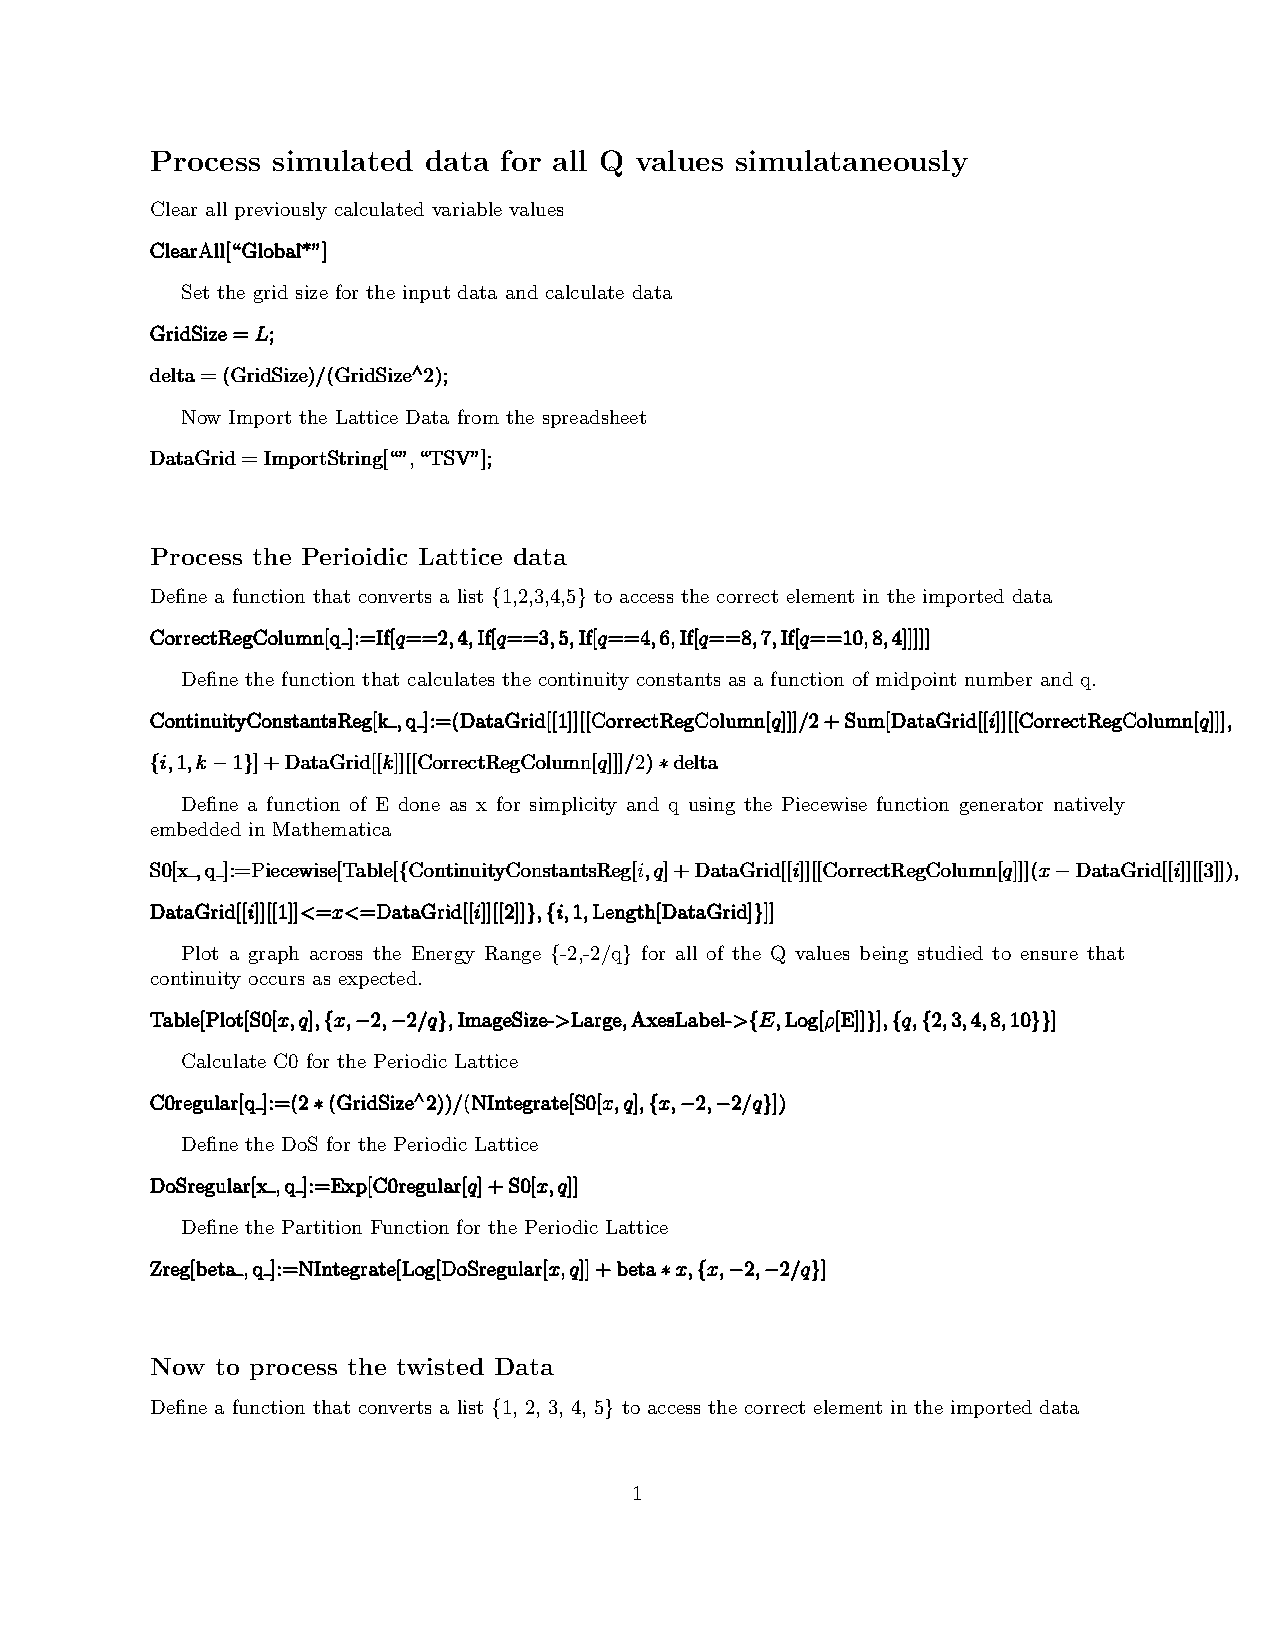
\includepdf[pages=-,scale=.8,pagecommand={}]{7-Appendices/AllQatOnceAnalysis.pdf}


% end Appendices

% begin References
\bibliographystyle{plain}
\bibliography{References}
% end Referecnes

% begin Acknowledgments
\renewcommand{\abstractname}{Acknowledgements}
\begin{abstract}
 I would like to thank,
 My friends and family for keeping me going throughout this challenging project.
 My project supervisor, without him, I wouldn't have made it as far as I did.
 My peers inside the Masters physics group whose collective ethos and support has provided invaluable insights over the last few years.
\end{abstract}
% end Acknowledgements

\end{document}
